\chapter{Probability and statistics}


\begin{description}
    \item[Probability]
        Model of a process where the underlying uncertainty is captured by random variables.
    \item[Statistics] 
        Determines the underlying process that explains an observation.
\end{description}


\section{Probability}
\begin{description}
    \item[State space] \marginnote{State space}
        Set $\Omega$ of all the possible results of an experiment.
        \begin{example}
            A coin is tossed two times. 
            $\Omega = \{ (\text{T}, \text{T}), (\text{T}, \text{H}), (\text{H}, \text{T}), (\text{H}, \text{H}) \}$
        \end{example}

    \item[Event] \marginnote{Event}
        Set of possible results (i.e. $A$ is an event if $A \subseteq \Omega$)

    \item[Probability] \marginnote{Probability}
        Let $\mathcal{E}$ be the set of all the possible events (i.e. power set of $\Omega$).
        The probability of an event is a function:
        \[ \prob{A}: \mathcal{E} \rightarrow [0, 1] \]
        \begin{example}
            Let $\Omega$ be as above.
            Given an event $A = \{ (\text{T}, \text{H}), (\text{H}, \text{T}) \}$, 
            its probability is: $\prob{A} = \frac{2}{4} = \frac{1}{2}$
        \end{example}

    \item[Conditional probability] \marginnote{Conditional probability}
        Probability of an event $B$, knowing that another event $A$ happened:
        \[ \prob{B \vert A} = \frac{\prob{A \cap B}}{\prob{A}} \text{, with } \prob{A} \neq 0 \]

        \begin{example}
            A coin is tossed three times. 
            Given the events $A = \{ \text{tails two times} \}$ and $B = \{ \text{one heads and one tails} \}$
            We have that:

            \begin{minipage}{\linewidth}
                \centering
                \small
                $\Omega = \{ 
                    (\text{T}, \text{T}, \text{T}), (\text{T}, \text{T}, \text{H}), (\text{T}, \text{H}, \text{T})
                    (\text{T}, \text{H}, \text{H}), (\text{H}, \text{T}, \text{T}), (\text{H}, \text{T}, \text{H})
                    (\text{H}, \text{H}, \text{T}), (\text{H}, \text{H}, \text{H})
                \}$
            \end{minipage}

            \begin{minipage}{.325\linewidth}
                \centering
                $\prob{A} = \frac{4}{8} = \frac{1}{2}$
            \end{minipage}
            \begin{minipage}{.325\linewidth}
                \centering
                $\prob{B} = \frac{6}{8} = \frac{3}{4}$
            \end{minipage}
            \begin{minipage}{.325\linewidth}
                \centering
                $\prob{A \cap B} = \frac{3}{8}$
            \end{minipage}

            \begin{minipage}{.48\linewidth}
                \centering
                $\prob{A \vert B} = \frac{3/8}{3/4} = \frac{1}{2}$
            \end{minipage}
            \begin{minipage}{.48\linewidth}
                \centering
                $\prob{B \vert A} = \frac{3/8}{1/2} = \frac{3}{4}$
            \end{minipage}
        \end{example}

    \item[Independent events] \marginnote{Independent events}
        Two events $A$ and $B$ are independent if:
        \[ \prob{A \cap B} = \prob{A}\prob{B} \]
        It follows that:

        \begin{minipage}{.48\linewidth}
            \centering
            $\prob{A \vert B} = \prob{A}$
        \end{minipage}
        \begin{minipage}{.48\linewidth}
            \centering
            $\prob{B \vert A} = \prob{B}$
        \end{minipage}

        In general, given $n$ events $A_1, \dots, A_n$, they are independent if:
        \[ \prob{A_1 \cap \dots \cap A_n} = \prod_{i=1}^{n} \prob{A_i} \]
\end{description}



\section{Random variables}
\begin{description}
    \item[Random variable (RV)] \marginnote{Random variable}
        A random variable $X$ is a function:
        \[ X: \Omega \rightarrow \mathbb{R} \]

    \item[Target space/Support] \marginnote{Target space}
        Given a random variable $X$, 
        the target space (or support) $\mathcal{T}_X$ of $X$ is the set of all its possible values:
        \[ \mathcal{T}_X = \{ x \mid x = X(\omega), \forall \omega \in \Omega \} \]
\end{description}


\subsection{Discrete random variables}

\begin{description}
    \item[Discrete random variable] \marginnote{Discrete random variable}
        A random variable $X$ is discrete if its target space $\mathcal{T}_X$ is finite or countably infinite.

        \begin{example}
            A coin is tossed twice.

            Given the random variable $X(\omega) = \{ \text{number of heads} \}$.
            We have that $\mathcal{T}_X = \{ 0, 1, 2 \}$, therefore $X$ is discrete.
        \end{example}

        \begin{example}
            Roll a die until 6 comes out.

            Given the random variable $Y(\omega) = \{ \text{number of rolls before 6} \}$.
            We have that $\mathcal{T}_Y = \{ 1, 2, \dots \} = \mathbb{N} \smallsetminus \{0\}$, 
            therefore $Y$ is discrete as $\mathcal{T}_Y$ is a countable set.
        \end{example}

    \item[Probability mass function (PMF)] \marginnote{Probability mass function (PMF)}
        Given a discrete random variable $X$, its probability mass function is a function $p_X: \mathcal{T}_X \rightarrow [0, 1]$ such that:
        \[ p_X(x) = \prob{X = x}, \forall x \in \mathcal{T}_X \]

        A PMF has the following properties:
        \begin{enumerate}
            \item $p_X(x) \geq 0, \forall x \in \mathcal{T}_X$
            \item $\sum_{x \in \mathcal{T}_X} p_X(x) = 1$
            \item Let $A \subseteq \Omega$, $\prob{X = x \in A} = \sum_{x \in A} p_X(x)$
        \end{enumerate}

        We denote with $X \sim p_X$ a random variable $X$ with PMF $p_X$.

        \begin{example}
            Let $\Omega = \{ (\text{T}, \text{T}), (\text{T}, \text{H}), (\text{H}, \text{T}), (\text{H}, \text{H}) \}$.
            Given a random variable $X = \{ \text{number of heads} \}$ with $\mathcal{T}_X = \{ 0, 1, 2 \}$.
            Its PMF is:
            \[
                \begin{split}
                    p_X &= \prob{X = 0} = \frac{1}{4} \\
                    p_X &= \prob{X = 1} = \frac{2}{4} \\
                    p_X &= \prob{X = 2} = \frac{1}{4}
                \end{split}  
            \]
        \end{example}
\end{description}


\subsection{Continuous random variables}

\begin{description}
    \item[Continuous random variable] \marginnote{Continuous random variable}
        A random variable $X$ is continuous if its target space $\mathcal{T}_X$ is uncountably infinite (i.e. a subset of $\mathbb{R}$).
        Usually, $\mathcal{T}_X$ is an interval or a union of intervals.

        \begin{example}
            Given a random variable $Z = \{ \text{Time before the arrival of a client} \}$.
            $Z$ is continuous as $\mathcal{T}_Z = [a, b] \subseteq [0, +\infty[$ is an uncountable set.
        \end{example}

    \item[Probability density function (PDF)] \marginnote{Probability density function (PDF)}
        Given a continuous random variable $X$, 
        its probability density function is a function $p_X: \mathcal{T}_X \rightarrow \mathbb{R}$ such that:
        \[ \prob{X \in A} = \int_{A} p_X(x) \,dx \]
        \[ \prob{a \leq X \leq b} = \int_{a}^{b} p_X(x) \,dx \]
        Note that $\prob{X = a} = \prob{a \leq X \leq a} = \int_{a}^{a} p_X(x) \,dx = 0$

        A PDF has the following properties:
        \begin{enumerate}
            \item $p_X(x) \geq 0, \forall x \in \mathcal{T}_X$ 
            \item $\int_{x \in  \mathcal{T}_X} p_X(x) \,dx = 1$
            \item $\prob{X \in A} =  \int_{A} p_X(x) \,dx$
        \end{enumerate}

        We denote with $X \sim p_X$ a random variable $X$ with PDF $p_X$.
    \end{description}



\section{Discrete joint distribution}

\begin{description}
    \item[Univariate distribution] \marginnote{Univariate distribution}
        Distribution with one random variable.
    
    \item[Multivariate distribution] \marginnote{Multivariate distribution}
        Distribution with multiple random variables.
    
    \item[Joint probability] \marginnote{Joint probability}
        Let $X$ and $Y$ be random variables respectively with target space $\mathcal{T}_X$ and $\mathcal{T}_Y$.
        The joint probability of $X$ and $Y$ has target space $\mathcal{T}_{XY} = \mathcal{T}_X \times \mathcal{T}_Y$
        and its PMF is:
        \[ p_{XY}(x_i, y_j) = \prob{X = x_i \cap Y = y_j} \]

        $p_X(x)$ and $p_Y(y)$ are the \textbf{marginal probabilities}. \marginnote{Marginal probability}

        \begin{example}
            Let $X$ and $Y$ be random variables respectively with five and three possible states.
            \begin{center}
                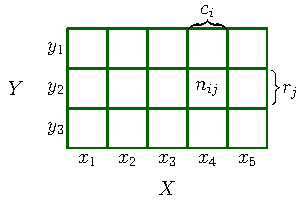
\includegraphics[width=0.4\textwidth]{img/_joint_probability_example.pdf}
            \end{center}
            We denote with:
            \begin{itemize}
                \item $N$ the number of events.
                \item $n_{ij}$ the number of events with state $X=x_i$ and $Y=y_j$ (i.e. $p_{XY}(x, y) = n_{ij}$).
                \item $c_i = \sum_{j=1}^{3} n_{ij}$ the sum of the $i$-th column.
                \item $r_j = \sum_{i=1}^{5} n_{ij}$ the sum of the $j$-th row.
            \end{itemize}

            The marginal probabilities are:\\
            \begin{minipage}{.48\linewidth}
                \centering
                \[ p_X(x_i) = \prob{X = x_i} = \frac{c_i}{N} \]
            \end{minipage}
            \begin{minipage}{.48\linewidth}
                \centering
                \[ p_Y(y_j) = \prob{Y = y_j} = \frac{r_j}{N} \]
            \end{minipage}

            The conditional probabilities can be computed as:
            \[ \prob{Y = y_j \vert X = x_i} = \frac{p_{XY}(x_i, y_i)}{p_X(x_i)} = \frac{n_{ij}/N}{c_i/N} = \frac{n_{ij}}{c_i} \]
            \[ \prob{X = x_i \vert Y = y_j} = \frac{p_{XY}(x_i, y_i)}{p_Y(y_j)} = \frac{n_{ij}/N}{r_j/N} = \frac{n_{ij}}{r_j} \]
        \end{example}
\end{description}



\section{Rules of probability}

\subsection{Sum rule}
\marginnote{Sum rule\\Marginalization property}
Given $X$ and $Y$ random variables. The sum rule states that:
\[
    p_X(\bm{x}) =
    \begin{cases}
        \sum_{\bm{y} \in \mathcal{T}_Y} p_{XY}(\bm{x}, \bm{y}) & \text{if } \bm{y} \text{ discrete} \\
        \int_{\mathcal{T}_Y} p_{XY}(\bm{x}, \bm{y}) \,d\bm{y} & \text{if } \bm{y} \text{ continuous}
    \end{cases}
\]

The sum rule relates the joint distribution and the marginal distribution.
In fact, the sum rule can be applied to any subset of the random variables of a joint distribution.
Given $\bm{x} = \begin{pmatrix} x_1, \dots, x_D \end{pmatrix}^T$, 
the marginal w.r.t. $x_i$ can be obtained by integrating/summing out all random variables except $x_i$:
\[ p(x_i) = \int p(x_1, \dots, x_D) \,d\bm{x}_{\smallsetminus i} \]

\subsection{Product rule}
\marginnote{Product rule}
\[ p(\bm{x}, \bm{y}) = p(\bm{y} \vert \bm{x}) p(\bm{x}) = p(\bm{x} \vert \bm{y}) p(\bm{y}) \]



\section{Bayes' theorem}
\begin{theorem}
    \marginnote{Bayes' theorem}
    Given two random variables $X$ and $Y$:
    \[
        \overbrace{p(\bm{x} \vert \bm{y})}^{\mathclap{\text{posterior}}} = 
            \frac
                { \overbrace{p(\bm{y} \vert \bm{x})}^{\mathclap{\text{likelihood }}}  \overbrace{p(\bm{x})}^{\mathclap{\text{ prior}}} }
                {\underbrace{p(\bm{y})}_{\mathclap{\text{evidence}}}} 
    \]
    where:
    \begin{descriptionlist}
        \item[Prior] \marginnote{Prior}
            is the prior knowledge of the unobserved data $\bm{x}$.

        \item[Likelihood] \marginnote{Likelihood}
            describes the relation between $\bm{x}$ and $\bm{y}$.

        \item[Posterior] \marginnote{Posterior}
            represents the quantity of interest (i.e. knowledge on $\bm{x}$ after observing $\bm{y}$).
        
        \item[Evidence/Marginal likelihood] \marginnote{Evidence/Marginal likelihood}
            normalizes the posterior. It is defined independently from $\bm{x}$ (i.e. is constant) as:
            \[ p(\bm{y}) = \int p(\bm{y} \vert \bm{x}) p(\bm{x}) \,d\bm{x} \]
    \end{descriptionlist}
\end{theorem}
\begin{proof}
    This is a direct consequence of the product rule:
    \[ 
        p(\bm{x} \vert \bm{y}) p(\bm{y}) = p(\bm{y} \vert \bm{x}) p(\bm{x}) \iff
        p(\bm{x} \vert \bm{y}) p(\bm{y}) = \frac{p(\bm{y} \vert \bm{x}) p(\bm{x})}{p(\bm{y})}
    \]
\end{proof}

Note: sometimes, instead of the full posterior, the maximum is considered (with loss of information):
\[ \max_x p(x \vert y) = \max_x \frac{p(y \vert x) p(x)}{\underbrace{p(y)}_{\mathclap{\text{constant}}}} = \max_x p(y \vert x) p(x) \]



\section{Statistics}

\begin{description}
    \item[Statistic] \marginnote{Statistic}
        A statistic of a random variable is a deterministic function defined on it. 
\end{description}


\subsection{Mean}
\begin{description}
    \item[Expected value (univariate)] \marginnote{Expected value (univariate)}
        Given a function $g$ of a random variable $X \sim p(x)$,
        its expected value is:
        \[ 
            \mathbb{E}_X[g(x)] = 
            \begin{cases}
                \sum_{x \in \mathcal{T}_X} g(x)p(x) & \text{if } $X$ \text{ is discrete} \\
                \int_{\mathcal{T}_X} g(x)p(x) \,dx  & \text{if } $X$ \text{ is continuous} \\
            \end{cases}
        \]

    \item[Expected value (multivariate)] \marginnote{Expected value (multivariate)}
        A multivariate random variable $X$ can be seen as 
        a vector of univariate random variables $\begin{pmatrix} X_1, \dots, X_D \end{pmatrix}^T$.
        Its expected value can be computed element wise as:
        \[ 
            \mathbb{E}_X[g(\bm{x})] = 
            \begin{pmatrix} \mathbb{E}_{X_1}[g(x_1)] \\ \vdots \\ \mathbb{E}_{X_D}[g(x_D)] \end{pmatrix} \in \mathbb{R}^D
        \]

    \item[Mean] \marginnote{Mean}
        Given a random variable $X \sim p(x)$,
        the mean of $X$ is its expected value with $g$ defined as the identity:
        \[ 
            \mathbb{E}_X[x] = 
            \begin{cases}
                \sum_{x \in \mathcal{T}_X} x \cdot p(x) & \text{if } $X$ \text{ is discrete} \\
                \int_{\mathcal{T}_X} x \cdot p(x) \,dx  & \text{if } $X$ \text{ is continuous} \\
            \end{cases}
        \]
\end{description}


\subsection{Variance}
\begin{description}
    \item[Covariance (univariate)] \marginnote{Covariance (univariate)}
        Given two univariate random variables $X$ and $Y$, their covariance is:
        \[ \text{Cov}_{XY}[x, y] = \mathbb{E}_{XY}[(x - \mathbb{E}_X[x])(y - \mathbb{E}_Y[y])] \]

        \begin{lemma} 
            $\text{Cov}_{XY}[x, y] = \mathbb{E}_{XY}[x, y] - \mathbb{E}_{X}[x]\mathbb{E}_{Y}[y]$
        \end{lemma}

    \item[Variance (univariate)] \marginnote{Variance (univariate)}
        The variance of a univariate random variable is given by:
        \[ \mathbb{V}_X[x] = \text{Cov}_X[x, x] \]
        Its square root is the standard deviation $\sigma(x)$.

    \item[Covariance (multivariate)] \marginnote{Covariance (multivariate)}
        Given two multivariate random variables 
        $X$ and $Y$ with states $\bm{x} \in \mathbb{R}^D$ and $\bm{y} \in \mathbb{R}^E$,
        their covariance is:
        \[ 
            \text{Cov}_{XY}[\bm{x}, \bm{y}] = \text{Cov}_{XY}[\bm{y}, \bm{x}]^T =
            \mathbb{E}_{XY}[\bm{xy}^T] - \mathbb{E}_{X}[\bm{x}]\mathbb{E}_{Y}[\bm{y}]^T \in \mathbb{R}^{D \times E}
        \]


    \item[Variance (multivariate)] \marginnote{Variance (multivariate)}
        Given a multivariate random variable $X$ with 
        states $\bm{x} \in \mathbb{R}^D$ and mean vector $\bm{\mu} \in \mathbb{R}^D$.
        Its variance is given by:
        \[
            \begin{split}
                \mathbb{V}_X[\bm{x}] &= \text{Cov}_X[\bm{x}, \bm{x}] \\
                    &= \mathbb{E}_X[\bm{xx}^T] - \mathbb{E}_X[\bm{x}]\mathbb{E}_X[\bm{x}]^T \\
                    &= 
                    \begin{pmatrix}
                        \text{Cov}[x_1, x_1] & \text{Cov}[x_1, x_2] & \cdots & \text{Cov}[x_1, x_D] \\
                        \text{Cov}[x_2, x_1] & \text{Cov}[x_2, x_2] & \cdots & \text{Cov}[x_2, x_D] \\
                        \vdots & \vdots & \ddots & \vdots \\
                        \text{Cov}[x_D, x_1] & \text{Cov}[x_D, x_2] & \cdots & \text{Cov}[x_D, x_D] \\
                    \end{pmatrix} \in \mathbb{R}^{D \times D}
            \end{split}
        \]
        This matrix is called covariance matrix and is symmetric positive semidefinite.

    \item[Correlation] \marginnote{Correlation}
        Given two random variables $X$ and $Y$, their correlation is:
        \[ \text{corr}[x, y] = \frac{\text{Cov}[x, y]}{\sqrt{\mathbb{V}[x]\mathbb{V}[y]}} \in [-1, 1] \]
        \begin{itemize}
            \item When $\text{corr}[x, y] \rightarrow +1$, $x$ and $y$ are expected to grow together.
            \item When $\text{corr}[x, y] \rightarrow -1$, $x$ grows when $y$ decreases and vice versa.
            \item When $\text{corr}[x, y] \rightarrow 0$, $x$ and $y$ are not correlated.
        \end{itemize}
\end{description}


\subsection{Empirical mean and variance}
In practice, it is not always possible to compute statistics on the real population.
Empirical observations can be made on a (finite) subset of the real population sampled as 
a finite number of identical random variables $X_1, \dots, X_N$.

\begin{description}
    \item[Empirical mean] \marginnote{Empirical mean}
        \[ \bar{x} = \frac{1}{N} \sum_{n=1}^{N}x_n \]
    \item[Empirical variance] \marginnote{Empirical variance}
        \[ \sigma^2 = \frac{1}{N} \sum_{n=1}^{N}(x_n - \bar{x})^2 \]
\end{description}



\section{Random variables properties}

\subsection{Manipulations}
\begin{itemize}
    \item $\mathbb{E}[\bm{x} + \bm{y}] = \mathbb{E}[\bm{x}] + \mathbb{E}[\bm{y}]$
    \marginnote{Manipulations of random variables}
    \item $\mathbb{E}[\bm{x} - \bm{y}] = \mathbb{E}[\bm{x}] - \mathbb{E}[\bm{y}]$
    \item $\mathbb{V}[\bm{x} + \bm{y}] = \mathbb{V}[\bm{x}] + \mathbb{V}[\bm{y}] + \text{Cov}[\bm{x}, \bm{y}] + \text{Cov}[\bm{y}, \bm{x}]$
    \item $\mathbb{V}[\bm{x} - \bm{y}] = \mathbb{V}[\bm{x}] + \mathbb{V}[\bm{y}] - \text{Cov}[\bm{x}, \bm{y}] - \text{Cov}[\bm{y}, \bm{x}]$
\end{itemize}


\subsection{Statistical independence}
\marginnote{Statistical independence}
Two random variables $X$ and $Y$ are statistically independent iff:
\[ p(\bm{x}, \bm{y}) = p(\bm{x})p(\bm{y}) \]

\begin{theorem}
    If $X$ and $Y$ are statistically independent, then:
    \begin{itemize}
        \item $p(\bm{x} \vert \bm{y}) = p(\bm{x})$ and $p(\bm{y} \vert \bm{x}) = p(\bm{y})$
        \item $\mathbb{V}_{XY}[\bm{x} + \bm{y}] = \mathbb{V}_X[\bm{x}] + \mathbb{V}_Y[\bm{y}]$
        \item $\text{Cov}_{XY}[\bm{x}, \bm{y}] = \nullvec$
    \end{itemize}
\end{theorem}


\subsection{Conditional independence}
\marginnote{Conditional independence}
Two random variables $X$ and $Y$ are conditionally independent given $Z$ iff:
\[ p(\bm{x}, \bm{y} \vert \bm{z}) = p(\bm{x} \vert \bm{z}) p(\bm{y} \vert \bm{z}) \, \forall \bm{z} \in \mathcal{T}_Z \]


\subsection{Inner product}
\marginnote{Inner product of random variables}
Given two zero mean random variables $X$ and $Y$, their inner product is defined as:
\[ \left\langle X, Y \right\rangle = \text{Cov}[x, y] \]
The covariance matrix is symmetric positive definite.

Moreover, we have that:
\begin{itemize}
    \item $\Vert X \Vert = \sqrt{\langle X, X \rangle} = \sqrt{\text{Cov}[x, x]} = \sqrt{\mathbb{V}[x]} = \sigma[x]$
    \item 
        $\cos\theta = \frac{\langle X, Y \rangle}{\Vert X \Vert \cdot \Vert Y \Vert} = 
        \frac{\text{Cov}[x, y]}{\sqrt{\mathbb{V}[x]\mathbb{V}[y]}}$, where $\theta$ is the angle between $X$ and $Y$.
    \item $X \perp Y \iff \langle X, Y \rangle = 0 \iff \text{Cov}[x, y] = 0 \iff X \text{ and } Y \text{ uncorrelated}$
\end{itemize}



\section{Common distributions}

\subsection{Discrete random variables}
\begin{descriptionlist}
    \item[Uniform distribution] \marginnote{Uniform distribution}
        Given a discrete random variable $X$ with $\vert \mathcal{T}_X \vert = N$,
        $X$ has an uniform distribution if:
        \[ p_X(x) = \frac{1}{N}, \forall x \in \mathcal{T}_X \]
    
    \item[Poisson distribution] \marginnote{Poisson distribution}
        Given a discrete random variable $X$ with mean $\lambda$,
        $X$ has a poisson distribution if:
        \[ p_X(x) = e^{-\lambda} \frac{\lambda^x}{x!}, \forall x \in \mathcal{T}_X \]

        A poisson distribution has $\mathbb{E}[x] = \lambda$ and $\mathbb{V}[x] = \lambda$.
\end{descriptionlist}


\subsection{Continuous random variables}
\begin{descriptionlist}
    \item[Continuous uniform distribution] \marginnote{Continuous uniform distribution}
        Given a continuous random variable $X$ with $\mathcal{T}_X = [a, b]$,
        $X$ has a continuous uniform distribution if:
        \[ p_X(x) = \frac{1}{b-a}, \forall x \in \mathcal{T}_X \]
    
    \item[Normal distribution] \marginnote{Normal distribution}
        Given a continuous random variable $X$ and the parameters $\mu$ (mean) and $\sigma$ (variance).
        $X$ has a normal distribution if:
        \[ p_X(x) = \frac{1}{\sigma \sqrt{2\pi}} e^{\frac{-(x-\mu)^2}{2\sigma^2}} , \forall x \in \mathcal{T}_X\]

        In the multivariate case, it is defined as:
        \[ 
            p(\bm{x}) = \mathcal{N}(\bm{x} \vert \bm{\mu}, \matr{\Sigma}) = 
                (2\pi)^{-\frac{D}{2}} \vert \matr{\Sigma} \vert^{-\frac{1}{2}} e^{(-\frac{1}{2}(\bm{x} - \bm{\mu})^T\matr{\Sigma}^{-1}(\bm{x}-\bm{\mu}))}
                \in \mathbb{R}
        \]
        where $\bm{\mu}$ is the mean vector and  $\matr{\Sigma}$ the covariance matrix.

        \begin{description}
            \item[Standard normal distribution] \marginnote{Standard normal distribution}
                Normal distribution with $\mu = 0$ and $\sigma = 1$ (univariate) or 
                $\bm{\mu} = \nullvec$ and $\matr{\Sigma} = \matr{I}$ (multivariate).
        \end{description}

        \begin{figure}[ht]
            \centering
            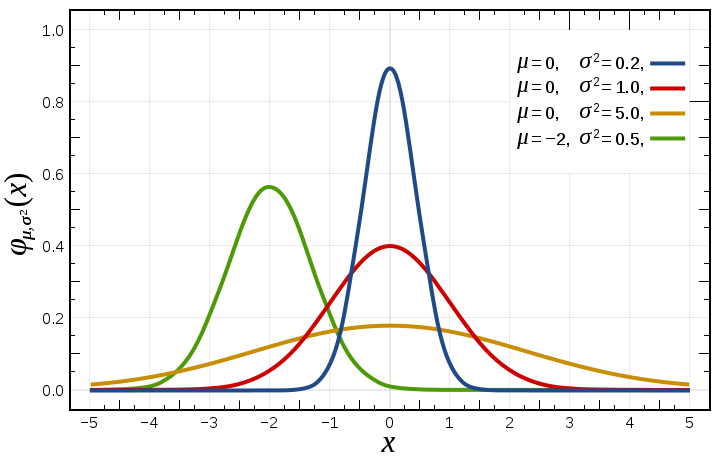
\includegraphics[width=0.40\textwidth]{img/normal_distribution.png}
            \caption{Normal distributions and standard normal distribution}
        \end{figure}


        \begin{theorem}[Linearity]
            \marginnote{Gaussian sum and linear transformations}
            Given $X$ and $Y$ independent Gaussian random variables with
            $p(\bm{x}) = \mathcal{N}(\bm{x} \vert \bm{\mu}_x, \matr{\Sigma}_x)$ and
            $p(\bm{y}) = \mathcal{N}(\bm{y} \vert \bm{\mu}_y, \matr{\Sigma}_y)$.
            It holds that:
            \[ p(a\bm{x} + b\bm{y}) = \mathcal{N}(a\bm{\mu}_x + b\bm{\mu}_y, a^2\matr{\Sigma}_x + b^2\matr{\Sigma}_y) \]
        \end{theorem}
\end{descriptionlist}